\documentclass[11pt]{article}

\usepackage[utf8]{inputenc}
\usepackage[margin=0.85in]{geometry}
\usepackage{graphicx}
\usepackage{booktabs}
\usepackage{longtable}
\usepackage{array}
\usepackage{hyperref}

\hypersetup{
  colorlinks=true,
  linkcolor=blue,
  citecolor=blue,
  urlcolor=blue
}
\graphicspath{{../figures/}}
\setlength{\parskip}{0.45em}
\setlength{\parindent}{0pt}

\title{Independent Axial Seamount Thermomechanical Model: Progress Report}
\author{Axial Modeling Project}
\date{October 2026}

\begin{document}
\maketitle

\begin{abstract}
This report records an independent PyLith implementation of the written
thermomechanical method for Axial Seamount, with observational checking against
authorized Ocean Observatories Initiative (OOI) records and raw BPR channels
from earlier Axial deployments, including MGDS-published tide corrections and
MPR drift corrections where available. It uses no Cabaniss model outputs,
eruption predictions, or published figure values. Published figure style,
layout, and explicit rheology labels inform project presentation and panel
mapping only. The project
verifies elastic and one-branch Maxwell responses, steady three-dimensional
heat conduction, temperature-property transfer, and postprocessed failure
connectivity, and synthetic three-branch historical forward checks. Central
and Eastern OOI histories provide 3,927 common finite daily records from 2014
through 2026; the aggregate quality code is retained as NOT EVALUATED. Original
raw NCEI BPR channels add deployments from 1987 through 2002, including the
1998 event, and raw MGDS channels add the 2002--04 Center record and further
records through 2022, including the 2011 event and post-eruption overlaps.
The 2002--04 South holdout has 0.658 m RMSE over 317 paired days. The first
one-branch OOI check applies a static-elastic pressure fit to
Maxwell mechanics and has a large Central displacement error. A separate
Maxwell-kernel inversion reduces Central RMSE to 0.005 m but leaves 0.225 m
Eastern holdout error. Raw 1998 and 2011 kernel checks leave South RMSE values
of 0.535 and 0.713 m. The historical three-branch event checks use synthetic
branch parameters and have held-out South biases of 0.329 m and 0.371 m.
Additional deployment checks span 1995–2022; the 2011–13 South comparison has
1.242 m RMSE and $-1.214$ m bias. The 2013–15 South 2 and South 1 checks have
0.358 m and 1.096 m RMSE, and the 2015–17 South 2 check has 0.265 m RMSE.
The 2018–20 South 2 and 2020–22 miniBPR South 1 checks have 0.105 m and
0.043 m RMSE across 741 and 648 paired days. Sixteen further raw MGDS station
holdouts span these three later windows; their RMSE values range from 0.031 m
to 0.705 m. Documented noise and sediment instability exclude two 2020–22
records, while the 2018–20 West BPR lacks a drift estimate and has 0.346 m
RMSE. These added spatial checks retain raw ocean and instrument effects and do
not calibrate the synthetic branches or static compliance.
Six additional 2017--18 raw MGDS stations are compared with OOI Central using a
static elastic ellipsoid response. Their RMSE values range from 0.106 to
0.575 m; tides, ocean variability, and unknown drift remain in the records, so
these are exploratory spatial checks.
The four-case temperature-dependent calibrations use the project-directed
linear 50-to-20 GPa modulus map. Raw BPR fits give 0.0926 m Center RMSE in
1998 and 0.1244 m in 2011; held-out South RMSE is 0.489--0.534 and
0.694--0.732 m. Fitted pressure minima reach $-95$ and $-72$ MPa. Both Center
fits include observed eruption deflation, so their connected-path histories
cannot independently predict eruption timing.
The corrected-observation event checks give 0.1154 m Center RMSE in 1998 and
0.1045 m in 2011, with held-out South RMSE of 0.632--0.680 and 0.709--0.745 m.
The 1998 channels have tide correction only; the 2011 Center channel also has
MPR drift correction, while South has tide correction only. Non-tidal ocean
variability remains, and the Center fits still include eruption deflation.
These outputs remain provisional: the ellipsoid compliance is not
mesh-converged, generalized Maxwell branch parameters are unavailable, the
owner-directed modulus interpolation is an assumption because Eq. 16 conflicts
with its stated modulus limits, and the written thermal equation specifies
zero heat production without mechanical feedback. The current work therefore
supports a partial implementation record, not a reproduction of the published
eruption forecasts.
\end{abstract}

\section{Scope and data provenance}

The project reconstructs model inputs from written descriptions of the study
and its supplement, then implements independent solvers and checks. The main
model article and publisher-served supplement are specification sources
[1, 2]. Independent raw OOI and Axial BPR observations and authorized MGDS
correction fields support model checks. Independent bathymetry, lava-flow
interpretations, earthquake locations, and seismic-velocity records support
the Figure 1 map [7--9]. Cabaniss model outputs, pressure/stress histories,
eruption predictions, source code, plotting scripts, and numerical figure
values are excluded. Published figures may inform visual style, layout, and
explicit rheology labels; their plotted results are not extracted or compared.
The supplement copy carries a confidential manuscript footer, so extracted
parameters remain version-qualified.

OOI daily BPR depth records cover Central and Eastern Caldera. The products
report relative uplift after detiding and drift correction; their aggregate
quality flag is NOT EVALUATED [4]. The analysis retains flag code 2 without
filtering. Common finite observations span 2014-09-05 through 2026-09-30. Raw
NCEI records provide uncorrected pressure from ten Axial deployments in
1987–96 and further deployments in 1997–99 and 2000–02. WC09–WC32 use 56.25-second
samples; WC51 onward uses 15-second samples. Selected MGDS files provide
original \texttt{Depth}, \texttt{RawDep}, and \texttt{RawDepth(m)} channels
from Center and South deployments between 2003 and 2022 [5, 6]. The 2020–22
miniBPR records are sampled every 100 seconds. The raw-data workflow excludes
derived detided, filtered, and pressure-drift-corrected fields. A separate
1998/2011 event check uses the archive's predicted-tide channel and the
combined tide/MPR-drift channel where available. Source files and processed
daily series remain outside version control. The MGDS archive uses the CC
BY-NC-SA 3.0 license, and its data citation and license are preserved in the
repository data notes.

\begin{figure}[htbp]
  \centering
  \begin{minipage}[t]{0.48\linewidth}
    \centering
    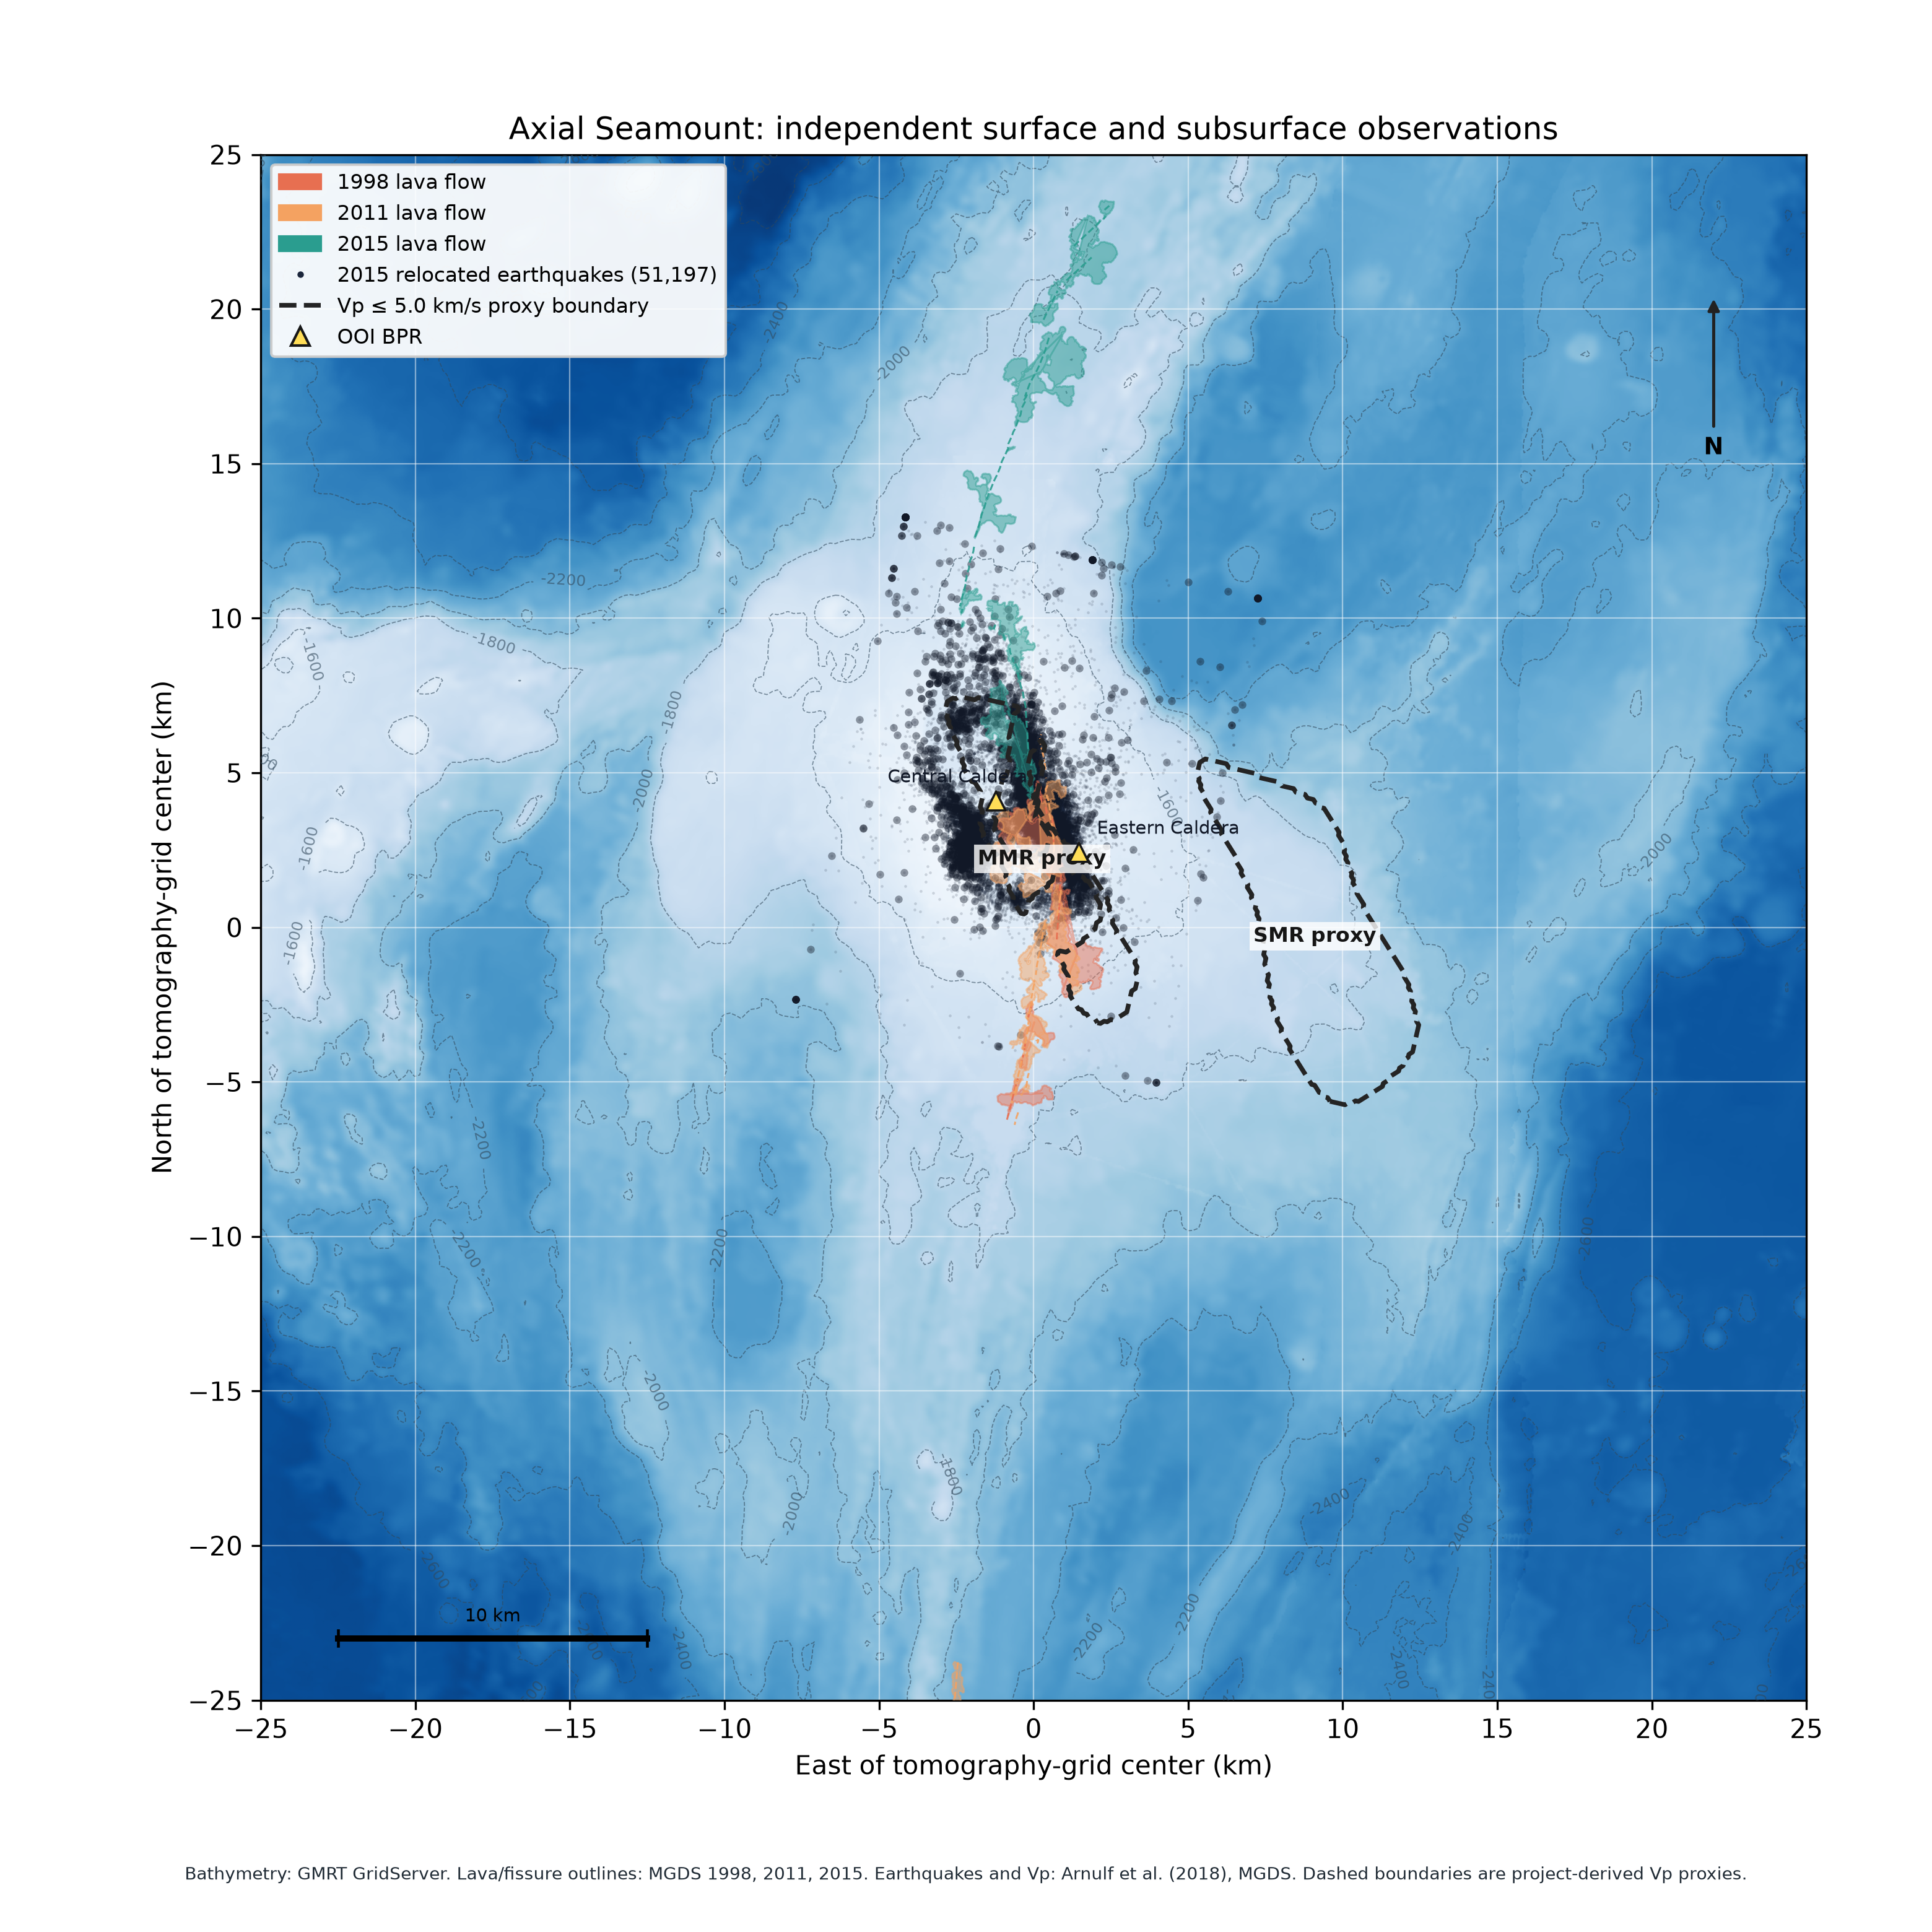
\includegraphics[width=\linewidth]{figure1_axial_geologic_map.png}

    \small (a) Independent Axial geology and seismic context.
  \end{minipage}\hfill
  \begin{minipage}[t]{0.48\linewidth}
    \centering
    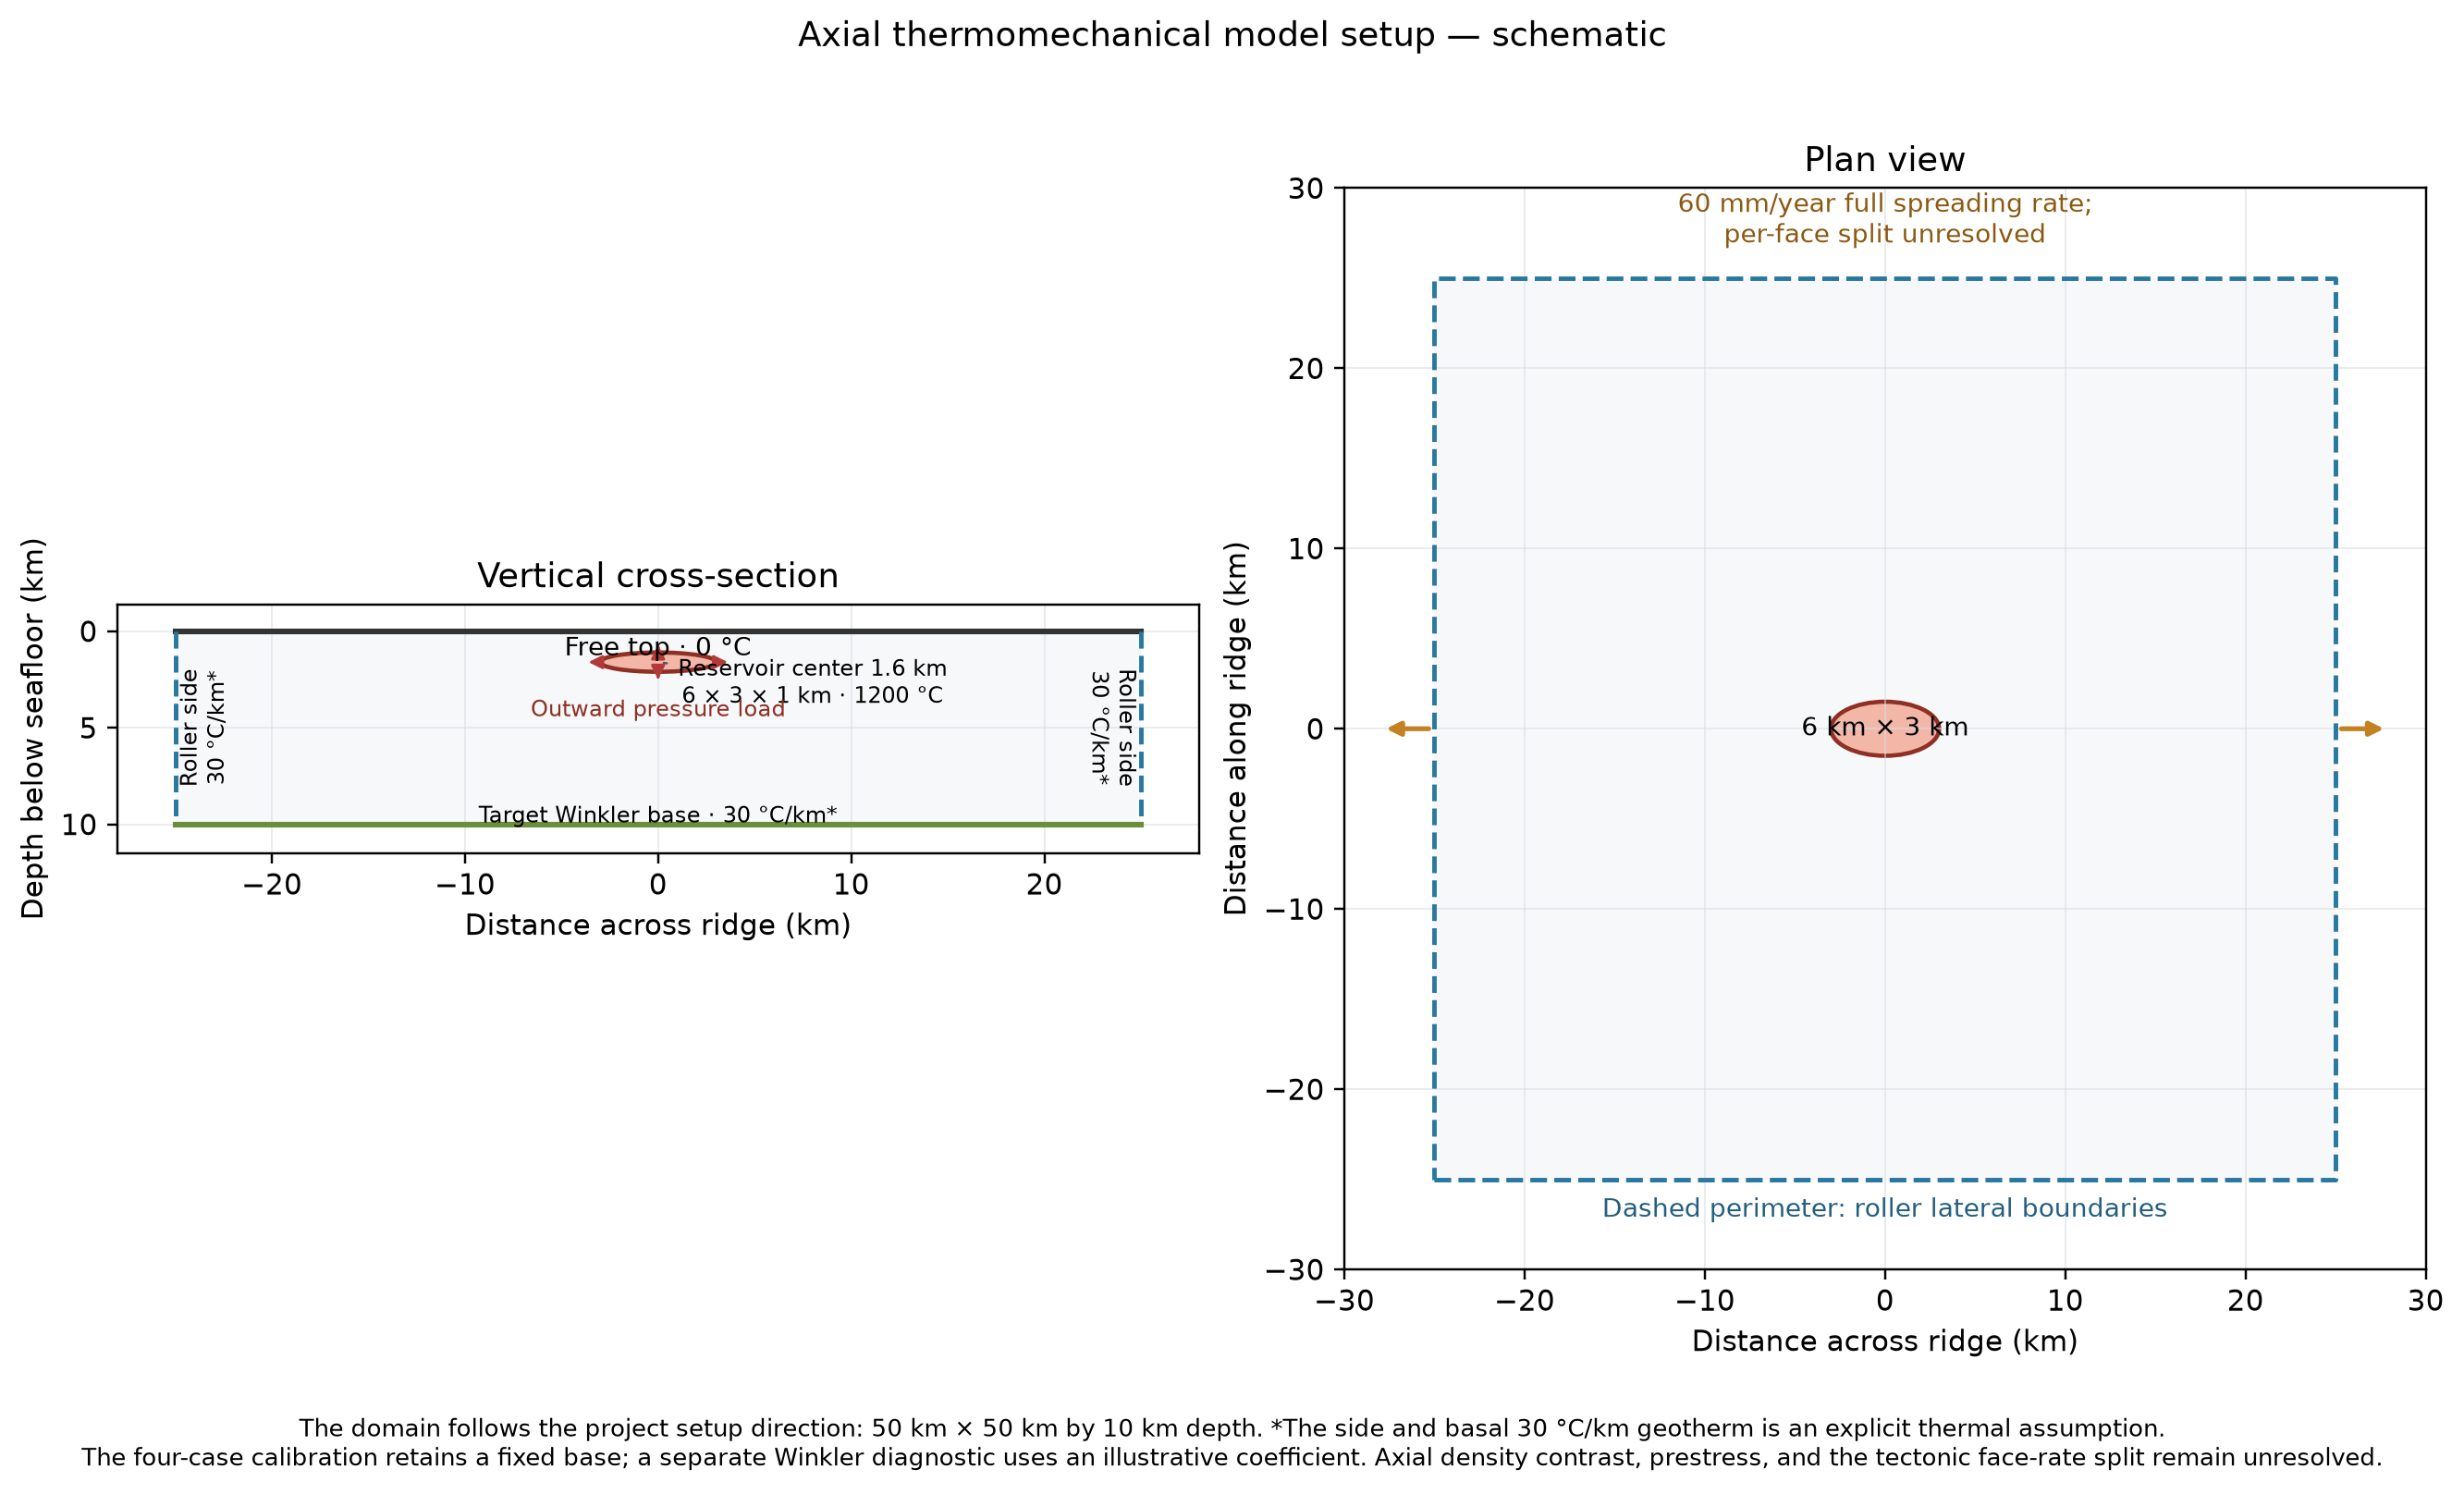
\includegraphics[width=\linewidth]{model_setup_schematic.png}

    \small (b) Project-directed model geometry and boundary conditions.
  \end{minipage}
  \caption{Project context and model setup assembled from independent data
  and project assumptions.}
  \label{fig:paper-figure-1}
\end{figure}

\section{Written model and implementation}

The specified reservoir is an ellipsoid measuring 6 by 3 by 1 km, centered
1.6 km below the seafloor. The written thermal method is steady conduction,
\begin{equation}
  \nabla\cdot(k\nabla T)=-Q, \qquad Q=0,
\end{equation}
with a 30 $^\circ$C/km background geotherm, a 0 $^\circ$C surface, and a
1200 $^\circ$C reservoir boundary. The hydrothermal conductivity law is
implemented as a separate case. Because lateral and basal thermal conditions
are not specified, the current finite-element calculation extends the
background geotherm to all outer faces and records this as an assumption.



The target base follows a Winkler foundation, where the restoring traction
scales with vertical displacement and an offset balances initial prestress.
PyLith's standard time-dependent Neumann condition accepts prescribed
tractions, not displacement feedback, so a separate static check updates basal
tractions from the solved displacement by outer iteration. A regional Juan de
Fuca gravity prior gives a finite coefficient of 32,373 Pa/m and a basal
prestress of 288.414 MPa for 6 km of 2,700 kg/m$^3$ crust above 4 km of
3,300 kg/m$^3$ mantle. The diagnostic applies gravity and that prestress with
a homogeneous 2,940 kg/m$^3$ density, preserving the integrated column load
while approximating the pressure profile with depth. Pressure and tectonic
increments are evaluated on the equilibrated reference stress. The spring
iteration uses a 1 Pa incremental-traction tolerance. This regional prior is
not an Axial measurement, the mesh is not converged, and the main pressure
calibrations retain a fixed base. The unit conversion and boundary check are
available with \texttt{make winkler-scale} and
\texttt{make winkler-foundation-check}.



\setcounter{figure}{2}
\begin{figure}[htbp]
  \centering
  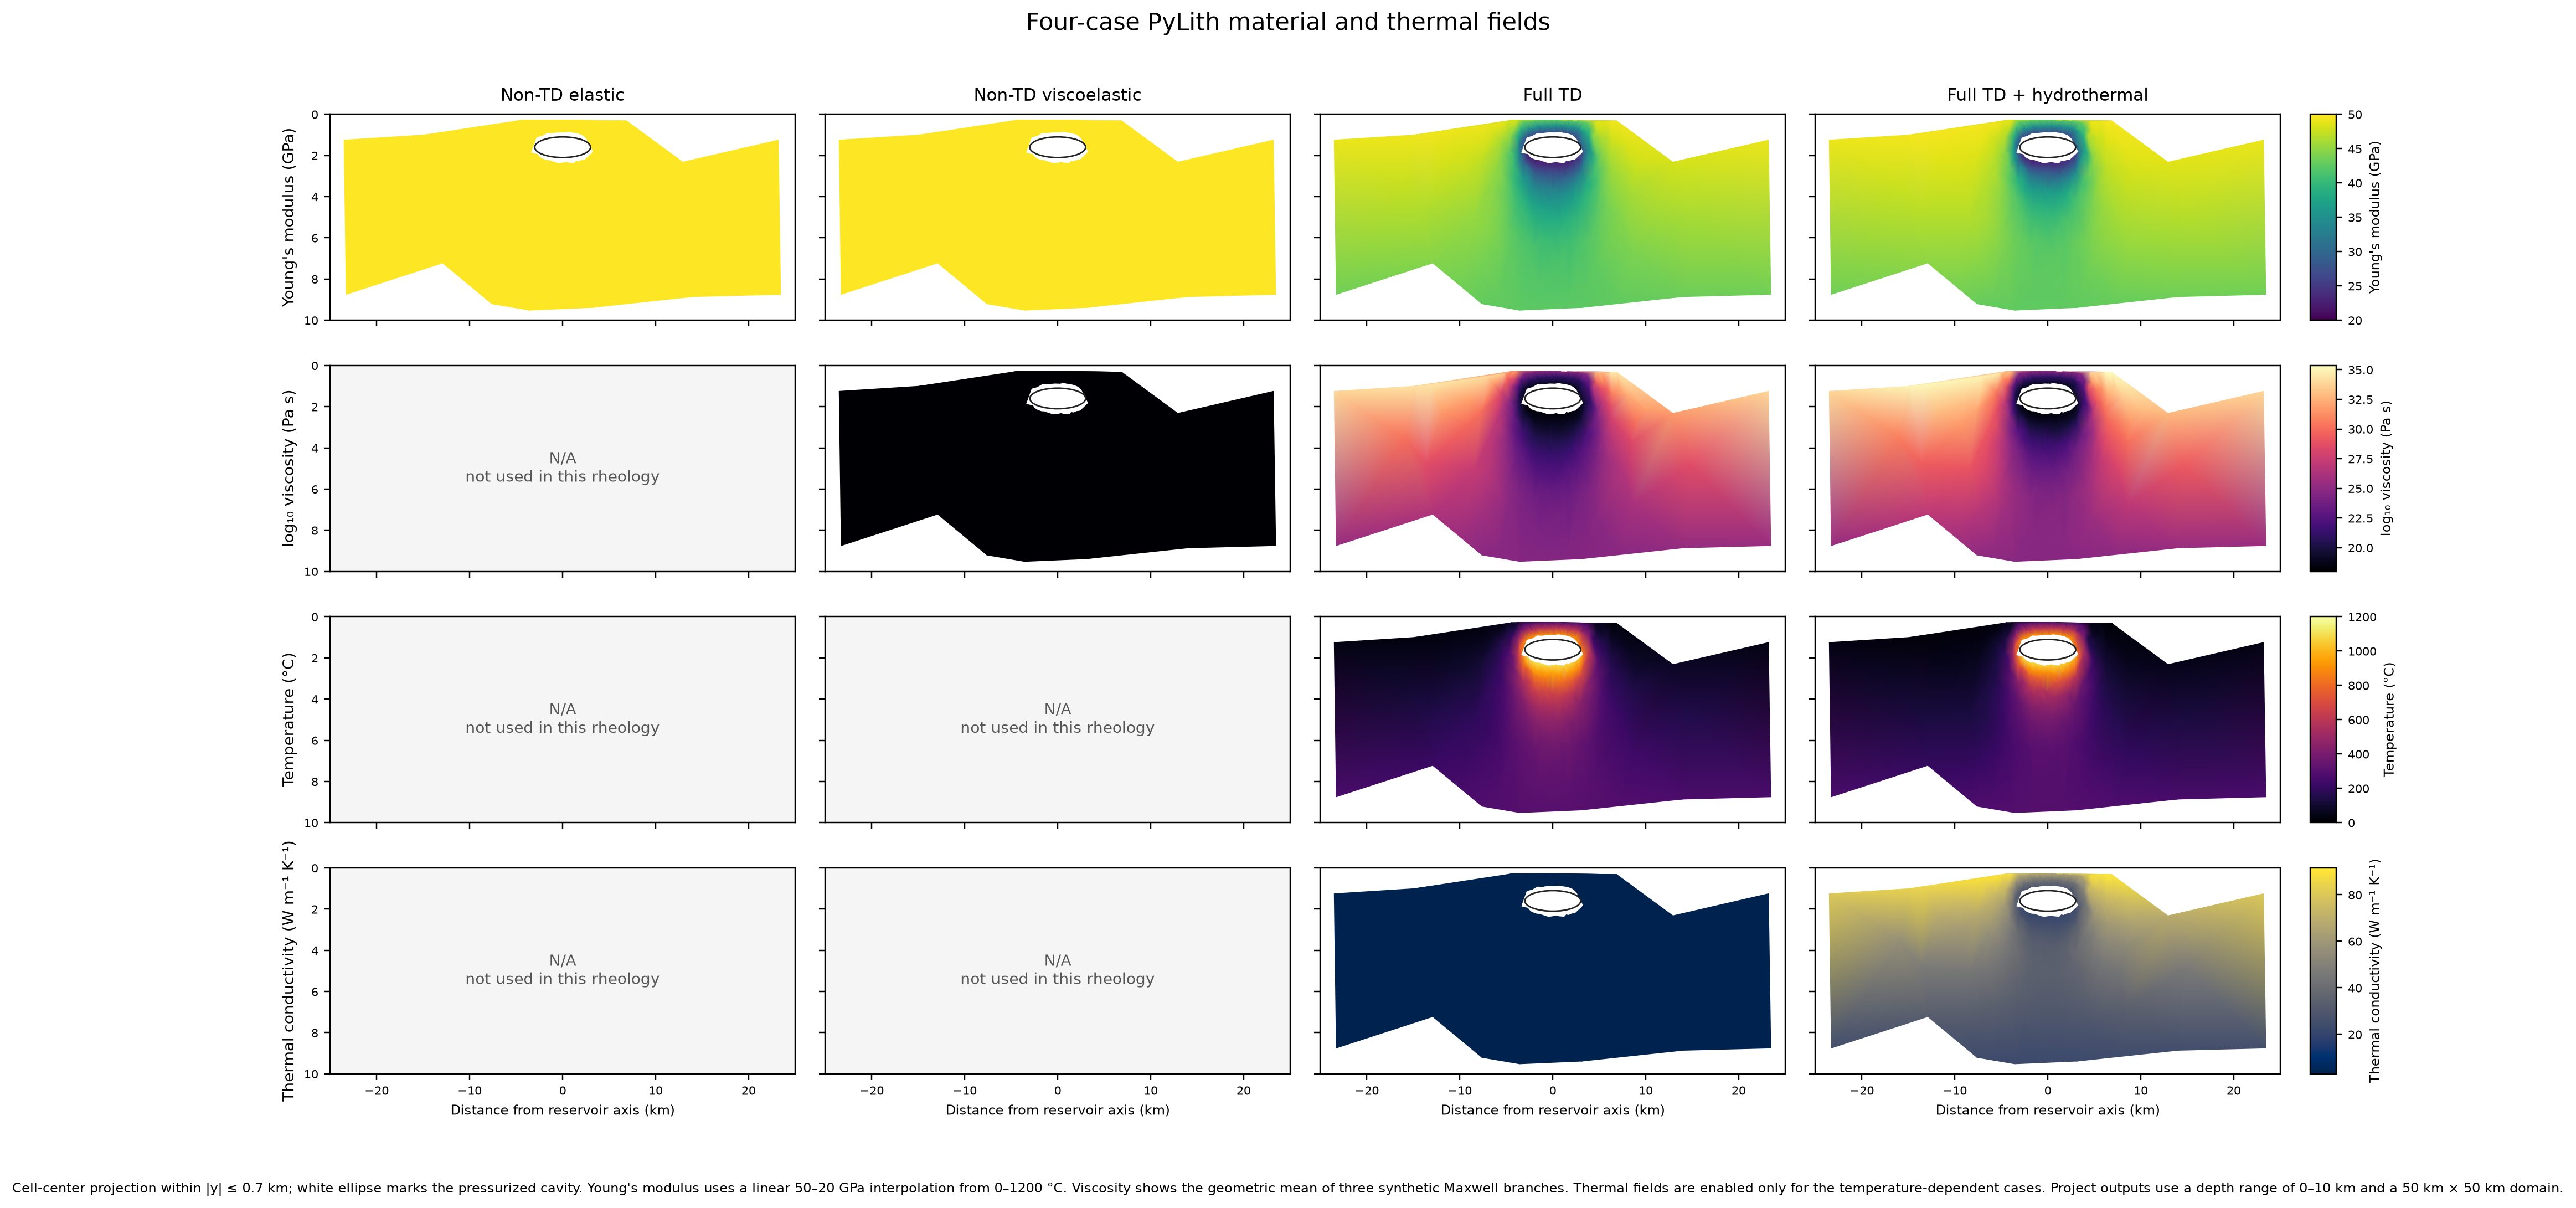
\includegraphics[width=0.98\linewidth]{figure3_rheology_property_matrix.png}
  \caption{Project-generated four-case property matrix arranged in a 4 by 4
  layout. Rows show Young's modulus, log viscosity, temperature, and thermal
  conductivity; columns are non-temperature-dependent elastic,
  non-temperature-dependent viscoelastic, Full TD, and Full TD plus
  hydrothermal cases. The 50-to-20 GPa modulus mapping follows the project
  instruction, while Maxwell branch viscosities are synthetic. The maps cover
  the project-directed 50 by 50 km horizontal box and 0--10 km depth. These are
  PyLith property fields used by the bounded common 1 MPa, two-year diagnostic
  run, not Cabaniss output or a calibrated eruption prediction. The solve uses
  a fixed base pending a validated Axial Winkler foundation. Generated by
  \texttt{make figure3-rheology-properties}.}
  \label{fig:four-case-properties}
\end{figure}

The Arrhenius viscosity law is evaluated from the temperature field. The
printed temperature-dependent Young's modulus equation increases from about
25 GPa toward 75 GPa as temperature rises, contrary to the written brittle
and ductile descriptions. The implementation preserves this equation only as
a diagnostic; it does not claim the trend is physically resolved. The written
Maxwell model requires a generalized branch spectrum that is not fully
specified. Current PyLith runs therefore use one Maxwell branch with explicitly
assumed properties. The PyLith 5.0.2 material interface supplies properties
and initial state through an auxiliary spatial database; a same-mesh restart
can transfer state when properties change [3].

The hydrothermal thermal solve now produces an exploratory midplane map of
temperature-dependent properties. This
slice uses the written Arrhenius viscosity and conductivity relations and
evaluates Eq. 16 exactly as printed. The finite-thickness slice, outer-face
geotherm, and incomplete generalized Maxwell spectrum limit comparison with
the complete four-rheology panels.



The hydrothermal Picard solve converges numerically on three independently
generated meshes with 2,761, 2,941, and 3,060 tetrahedra. Spatial changes do
not settle at 105 common host-rock probes: the 1,200-to-1,150 m pair has a
13.45 $^\circ$C probe RMSE and a 64.61 $^\circ$C maximum change, while the
1,150-to-1,100 m pair has a 35.55 $^\circ$C RMSE and a 324.29 $^\circ$C
maximum near the reservoir edge.
The mesh sequence is unstructured and non-nested, so these finite-probe
comparisons do not establish a volume norm or formal convergence. They show
that the current thermal field remains spatially sensitive near the reservoir.



The project has verified a three-dimensional steady heat solve, a synthetic
thermal-to-property-to-mechanics transfer, and same-mesh Maxwell restart. An
unchanged-property segmented run differs from a continuous run by at most
1.612$\times 10^{-8}$ in displacement, stress, total strain, and viscous strain.
A separate uniform 1200 $^\circ$C material swap carries viscous strain across
the restart boundary and changes the final displacement by 50.08 percent
relative to the uniform-property run. This verifies the restart interface;
the artificial uniform-temperature swap is not a coupled physical case.

A manufactured check transfers an affine temperature field from a
six-tetrahedron source mesh to the 2,761-tetrahedron mechanics mesh, with a
maximum interpolation error of $1.14\times10^{-13}\ ^\circ$C. The smoke case
also solves the written hydrothermal model on a distinct 3,060-tetrahedron
ellipsoid mesh. Sampling at mechanics-cell centers yields finite temperatures
from 8.769 to 1,066.240 $^\circ$C. PyLith completes a two-second Maxwell solve
using the mapped heterogeneous material database and writes finite stress and
viscous strain; peak stress is $1.75811\times10^7$ Pa. The smoke case verifies
point sampling of a physical steady field and material-database use across
meshes. It does not test conservative transfer, time-varying properties, or
two-way thermal-mechanical feedback.

The paper's thermal method specifies $Q=0$ and gives no stress- or
deformation-generated heat term. The roadmap's mechanics-to-thermal return
coupling therefore lacks a written physical law. The current one-way OOI
diagnostic does not add an invented heat source. This prevents a complete
two-way reproduction until the return coupling is specified or approved as a
separate exploratory extension.

\section{Independent observations and model checks}

Available Central and Eastern OOI uplift records cover the period described below. Each instrument uses its own first-sample reference. The plot is an
observation-only partial record: it has no raw pre-2014 values, eruption
markers, or earthquake counts.



The original raw NCEI channels add intermittent Axial deployment records from
1987 through 2002, while MGDS raw channels extend coverage from July 2002
through 2022. For the NeMO 2002--04 Center file, MGDS identifies its
\texttt{DriftCorrRawDep} field as unchanged because the recorded drift
correction was zero. The analysis excludes its tide-subtracted and filtered
fields. The
deployment-context figure places every deployment on its own first-sample
baseline; gaps between deployments are not interpolated, and no tide, ocean, or
sensor pressure-drift correction is applied. WC09–WC32 were sampled every
56.25 seconds; later NCEI and moored MGDS records use 15-second samples, while
the 2020–22 miniBPRs use 100-second samples. The unstable 2017–18 Center record
is displayed for context and excluded from model forcing.

An independent Fox archive from MGDS (IEDA/322344; doi:10.1594/IEDA/322344)
for the same 1997–98 Center and South instruments agrees with NCEI relative
uplift over 309 Center and 365 South days, with correlations above 0.999999 and
RMSE values of 0.050 and 0.016 m.
This checks raw-channel handling across archives; it does not add independent
station coverage. The archive's detided and low-pass-filtered fields are
excluded.



An elastic Mogi point source is calibrated to Central uplift and checked
against the Eastern record. The inferred pressure spans $-2.96$ to $+1.06$
GPa; Eastern RMSE is 0.0594 m with 0.995 correlation. The spatial correlation
does not validate this pressure scale. It shows that the point-source proxy
cannot supply the intended historical ellipsoid pressure model.

The raw historical channels add Center-to-South checks at the 1998 and 2011
eruptions, a 1995–96 pre-eruption overlap, and three later deployment overlaps.
The 1995–96 WC68/WC69 overlap spans 338 paired daily values. Its held-out South
prediction has 0.180 m RMSE, +0.159 m bias, and 0.876 correlation; the raw
record's slow South trend is not captured by the static model. The later pairs
span 614 paired
days in 2003–05, 572 in 2007–09, and 731 in 2011–13. Static Mogi predictions
have South RMSE values of 0.134, 0.156, and 0.387 m, with respective biases of
+0.113, +0.136, and +0.363 m. These channels retain tides, oceanographic
variability, and sensor drift, and the fits omit viscoelastic memory. They
extend observation checking across the pre-OOI interval; they are not
calibrated pressure histories or eruption forecasts.

The three-branch historical forward checks use first-common-day zeroing and
infer each daily pressure from the static Center compliance. In the 1998 pair,
the Center and held-out South RMSE values are 0.186 m and 0.503 m; the 2011
values are 0.114 m and 0.680 m. South biases are +0.329 m and +0.371 m,
respectively. From 2013–15, Center forcing predicts South 2 with 0.358 m RMSE;
South 1, held out independently, has 1.096 m RMSE and $-0.988$ m bias. The
2015–17 South 2 holdout has 0.265 m RMSE and $-0.245$ m bias. The inferred
pressure ranges reach $-50.7$ to $+26.7$ MPa and 0 to $+20.8$ MPa. These checks
use synthetic branch reference viscosities and fractions, retain raw ocean and
instrument effects, and inherit the nonconverged static compliance. They test
the historical loading path without calibrating rheology or producing a
hindcast.

The saved stress histories for all twelve raw-BPR-driven windows are also
evaluated with the current Mohr--Coulomb proxy: cohesion is 1 MPa, friction
angle is 25 degrees used directly as $\phi$, and pore pressure is zero. A
tensile cutoff is not applied to the shear path. The resulting
cavity-to-surface paths appear within the first 196 days of all twelve windows,
including the ten intervals without an eruption. In 2002--04, path onset is
bracketed at 53.64 days; its first saved path appears at day 56. In 1998 a path is already
present at the first saved output, so onset is only bounded above by seven
days. In 2011 linear stress interpolation brackets onset at 17.61 days after
the first common BPR day. The 2013–15 and 2015–17 paths appear at 34.75 days
and by the first saved day, respectively; the 2018–20 and 2020–22 paths first
appear at 21 and 35 days. The same proxy therefore fails to distinguish the
eruption windows from inter-eruption intervals and is not calibrated to
eruption timing. The written criterion also requires tensile failure at the
reservoir, but tensile strength is unspecified and is not assigned. At saved
records with a connected path, maximum cavity tension is 94.0 MPa in 1998 and
71.1 MPa in 2011, compared with 58.3 MPa across the ten inter-eruption
windows. Using unrounded output values, strengths in $(58.3221,71.0951]$ MPa
would separate these windows only for this saved-record diagnostic and its
synthetic branch properties, zero pore
pressure, direct friction interpretation, raw uncorrected channels, and
unconverged mesh. This conditional interval is not a measured or calibrated
rock strength. The joint condition is checked only at saved PyLith records.

\begin{table}[htbp]
  \centering
  \small
  \begin{tabular}{lrrr}
    \toprule
    BPR window & First path time & Saved records with a path & Max. tension on path (MPa) \\
    \midrule
    1995--96 & $\leq 7$ days & 46/49 & 6.08 \\
    2002--04 & 53.64 days & 30/46 & 6.94 \\
    1998 & $\leq 7$ days & 44/44 & 94.00 \\
    2003--05 & 25.38 days & 83/88 & 32.30 \\
    2005--07 & 195.84 days & 71/117 & 14.18 \\
    2007--09 & 67.86 days & 68/83 & 10.96 \\
    2011 & 17.61 days & 30/47 & 71.10 \\
    2011--13 & $\leq 7$ days & 105/106 & 58.32 \\
    2013--15 & 34.75 days & 96/102 & 50.50 \\
    2015--17 & $\leq 7$ days & 97/98 & 36.00 \\
    2018--20 & 21 days & 98/106 & 13.69 \\
    2020--22 & 35 days & 16/93 & 6.11 \\
    \bottomrule
  \end{tabular}
  \caption{Provisional joint failure diagnostics on the
  twelve historical three-branch stress histories. Time is measured from each
  independently zeroed BPR window. Thresholds use 1 MPa cohesion, 25-degree
  friction angle, and zero pore pressure. Maximum tension is the maximum
  cavity stress on saved records that also have a connected path; no tensile
  strength is assigned. Onsets
  after the first saved record are interpolated linearly between saved PyLith
  stress records; paths already present in the first output are bounded by
  seven days.}
  \label{tab:historical-failure-path}
\end{table}

A bounded time-step refinement shows that these first-path estimates depend on
the integration interval. In the 2011 history, the interpolated first crossing
moves from 17.61 days at seven-day steps to 2.29 days at one day and 2.28 days
at half- and quarter-day steps. The 2002--04 quiet-period estimate shifts from
53.64 days at seven-day steps to 26.94 days at one day and 26.93 days at
half- and quarter-day steps. The full 80-day quarter-day cases completed within
the five-minute per-run limit. At finer steps, both paths appear and disappear
repeatedly. These results show that coarse
sampling misses short-lived paths, while the refined first crossing remains a
diagnostic under synthetic branches, static pressure compliance, and the
nonconverged mesh, not a sustained eruption time.

A 27-case Mohr--Coulomb sweep reuses the twelve saved historical stress
histories and varies cohesion from 1 to 10 MPa, friction angle from 15 to
35 degrees, and pore pressure from 0 to 25 MPa. The fraction of saved records
with a connected cavity-to-surface path ranges from 64 to 100 percent for
1998 and 36 to 100 percent for 2011. These parameter combinations are
diagnostic scenarios; only the 1 MPa, 25-degree, zero-pressure case matches
the existing proxy. The deployment windows are not negative eruption controls,
and the occupancy fractions do not measure prediction accuracy.





The 2011 raw-BPR check also carries one three-branch Maxwell stress history
from the September 2010 event overlap through the August 2013 replacement
deployment. The Center records do not overlap and have a five-day gap, so the
run holds inferred pressure at its terminal pre-gap value and baselines each
instrument segment independently. The event South holdout has 0.680 m RMSE,
+0.371 m bias, and 0.997 correlation. The 2011--13 South holdout has 1.246 m
RMSE, $-1.217$ m bias, and 0.991 correlation. This shared slow trend does not
remove the large holdout bias; the result remains provisional under synthetic
branches, raw uncorrected channels, and nonconverged compliance.



The 1998 check carries one three-branch Maxwell stress history from the
October 1997 WC81/WC82 overlap through May 1999. The original WC81 Center
channel ends on 7 August 1998; the run then holds terminal inferred pressure
constant for 270 days while the WC82 South station continues. The 309-day
event South holdout has 0.503 m RMSE, +0.329 m bias, and 0.995 correlation.
After the Center record ends, the independently baselined South holdout has
0.063 m RMSE and -0.369 correlation. Its low RMSE reflects the small amplitude
of the nearly flat model and raw follow-up record, not evidence of predictive
skill. The continued pressure is an explicit assumption, and the result
remains provisional under synthetic branches and nonconverged compliance.



Ten additional raw Center/South overlaps extend the three-branch check across
1995–2022. Table~\ref{tab:historical-generalized-maxwell} summarizes the
held-out South comparisons. Each window has its own first-day zero, and
deployment gaps are left unfilled. The 2011–13 correlation of 0.991 coexists
with a 1.242 m RMSE and $-1.214$ m bias. Large residuals, changing correlations,
synthetic branch parameters, and uncorrected records prevent these plots from
establishing a historical calibration.

\begin{table}[htbp]
  \centering
  \small
  \begin{tabular}{lrrr}
    \toprule
    Interval & RMSE (m) & Bias (m) & Correlation \\
    \midrule
    1995--96 & 0.183 & $-0.161$ & 0.793 \\
    2002--04 & 0.658 & $-0.655$ & 0.366 \\
    2003--05 & 0.651 & $-0.649$ & 0.660 \\
    2005--07 & 0.157 & $-0.135$ & 0.958 \\
    2007--09 & 0.123 & $-0.101$ & $-0.355$ \\
    2011--13 & 1.242 & $-1.214$ & 0.991 \\
    2013--15 & 0.358 & $-0.089$ & 0.991 \\
    2015--17 & 0.265 & $-0.245$ & 0.973 \\
    2018--20 & 0.105 & $-0.096$ & 0.787 \\
    2020--22 & 0.043 & $-0.017$ & 0.788 \\
    \bottomrule
  \end{tabular}
  \caption{Held-out South residuals for ten raw deployment overlaps.}
  \label{tab:historical-generalized-maxwell}
\end{table}

The same model runs also predict three additional raw BPR locations that were
not used to define their primary Center/South pairs. WC67 is held out from the
1995--96 WC68-driven run over 338 days; NeMO South 1 is held out from the
2007--09 Center-driven run over the 572 days shared with the primary window.
The 2013–15 South 1 record adds a 711-day holdout. The WC67 residual is small;
the later South holdouts have larger errors, including the 2013–15 South 1
bias of $-0.988$ m. These differences show that spatial transfer varies across
deployments and that every raw channel remains a separate model check.

\begin{table}[htbp]
  \centering
  \small
  \begin{tabular}{lrrrr}
    \toprule
    Held-out raw station & Window & RMSE (m) & Bias (m) & Correlation \\
    \midrule
    WC67 & 1995--96 & 0.036 & $-0.021$ & 0.685 \\
    NeMO South 1 & 2007--09 & 0.221 & $-0.191$ & $-0.506$ \\
    NeMO South 1 & 2013--15 & 1.096 & $-0.988$ & 0.985 \\
    \bottomrule
  \end{tabular}
  \caption{Additional independent BPR station checks using the existing
  Center-driven Maxwell solutions. Neither station contributes to the pressure
  history used in its model run.}
  \label{tab:additional-historical-bpr-stations}
\end{table}

Sixteen further raw MGDS stations add holdouts to the 2015--17, 2018--20, and
2020--22 Center-driven solutions. Each station and its Center comparison are
zeroed on their first shared day. The model uses only original
\texttt{RawDep}, \texttt{RawDepth(m)}, or \texttt{Depth} channels; no data
product associated with Cabaniss et al. enters the comparison. Raw ocean
variability and drift remain. AX-105 in 2018--19 has no linear drift correction
in the source file; the 2018--20 West record has no MPR-based drift estimate.
Unknown drift remains in the 2020--22 East and North records. The 2018--20 North
record is omitted because its archived coordinates conflict with its source
location note. AX-303 in 2020--22 is excluded from metrics for its documented
high-noise interval, and BPR West is excluded for documented sediment-site
instability.

\begin{table}[htbp]
  \centering
  \scriptsize
  \begin{tabular}{llrrrr}
    \toprule
    Held-out raw station & Window & Days & RMSE (m) & Bias (m) & Correlation \\
    \midrule
    AX-302 Trevi & 2015--17 & 687 & 0.211 & $-0.189$ & 0.984 \\
    AX-307 Magnesia West & 2015--17 & 687 & 0.496 & $-0.465$ & 0.994 \\
    AX-308 South 1 & 2015--17 & 605 & 0.280 & $-0.256$ & 0.982 \\
    AX-106 Ashes & 2015--17 & 687 & 0.705 & $-0.666$ & 0.993 \\
    AX-303 Marker 33 & 2015--17 & 687 & 0.213 & $-0.190$ & 0.942 \\
    AX-105 South Pillow Mound & 2015--17 & 687 & 0.293 & $-0.255$ & 0.544 \\
    AX-307 Magnesia West & 2018--20 & 310 & 0.118 & $-0.096$ & 0.792 \\
    AX-302 Trevi & 2018--20 & 308 & 0.034 & $-0.016$ & 0.778 \\
    AX-105 South Pillow Mound & 2018--20 & 302 & 0.039 & +0.012 & 0.138 \\
    BPR West Rim$^*$ & 2018--20 & 739 & 0.346 & +0.305 & $-0.267$ \\
    AX-105 South Pillow Mound & 2020--22 & 648 & 0.180 & +0.174 & 0.174 \\
    AX-302 Trevi & 2020--22 & 648 & 0.031 & $-0.014$ & 0.722 \\
    AX-104 Bag City & 2020--22 & 647 & 0.047 & +0.031 & 0.554 \\
    AX-307 Magnesia West & 2020--22 & 647 & 0.031 & $-0.002$ & 0.791 \\
    BPR East$^\dagger$ & 2020--22 & 647 & 0.132 & +0.109 & $-0.163$ \\
    BPR North$^\dagger$ & 2020--22 & 641 & 0.486 & $-0.483$ & 0.680 \\
    \bottomrule
  \end{tabular}
  \caption{Additional held-out MGDS stations using the existing synthetic
  three-branch Maxwell histories. All stations remain uncorrected raw
  observations. $^*$No MPR-based drift estimate is available for the 2018--20
  West record. $^\dagger$Drift is unknown for the 2020--22 full-size BPRs.}
  \label{tab:supplemental-raw-bpr-stations}
\end{table}

Six original MGDS BPR records from 2017--18 are held out against OOI Central.
Each station and the OOI series are zeroed at the first shared day; OOI quality
codes are retained without filtering. The static elastic prediction scales
Central uplift by the PyLith compliance at each station. No tide, ocean, or
instrument-drift corrections are applied. MGDS reports repeated offsets at
AX-105 from 25 November through 11 December 2017, so those 17 days are omitted
from its primary metrics. The data remain original \texttt{RawDepth} or
\texttt{Depth} channels from IEDA/322282, distributed under CC BY-NC-SA 3.0.

\begin{table}[htbp]
  \centering
  \small
  \begin{tabular}{lrrrrr}
    \toprule
    Held-out raw station & Paired days & Primary days & RMSE (m) & Bias (m) & Correlation \\
    \midrule
    AX-303 Marker 33 & 387 & 387 & 0.475 & $-0.445$ & 0.958 \\
    AX-105 South Pillow Mound & 385 & 368 & 0.575 & $-0.497$ & 0.883 \\
    AX-302 Trevi & 389 & 389 & 0.106 & $-0.092$ & 0.961 \\
    AX-307 Magnesia West & 386 & 386 & 0.474 & $-0.453$ & 0.976 \\
    NeMO North & 383 & 383 & 0.341 & $-0.333$ & 0.944 \\
    NeMO West & 388 & 388 & 0.341 & +0.309 & $-0.890$ \\
    \bottomrule
  \end{tabular}
  \caption{2017--18 original raw MGDS station checks against OOI Central.
  Predictions use a static elastic ellipsoid with station-specific surface
  compliance. AX-105 primary metrics omit MGDS-reported offsets. Raw tides,
  ocean variability, and instrument drift remain in all station series.}
  \label{tab:ooi-2017-2018-raw-bpr-holdouts}
\end{table}











\clearpage

The elastic ellipsoid comparison improves the pressure scale but remains
mesh-sensitive. On the 2,761-tetrahedron mesh, unit-load compliance is
0.0318994 m/MPa at Central and 0.00345580 m/MPa at Eastern. The static
Central-calibrated pressure spans $-62.21$ to 22.16 MPa. Eastern RMSE is
0.221 m, relative L2 error is 76.36 percent, and correlation is 0.995.
Across tested refinements, station compliance changes by 21--76 percent;
these results do not establish a stable pressure calibration. The bounded
station-region comparison uses 2,761, 3,031, 3,124, 3,053, and 3,325
tetrahedra. These independently generated unstructured meshes are not
guaranteed to be nested: the 950 m case has fewer elements than the 1,000 m
case and changes Central and Eastern compliance by 59.8 and 58.1 percent. The
900 m case then changes them by $-35.1$ and
$-31.5$ percent. Repeating the five solves reproduced their results exactly,
but the sequence has no compliance plateau and no adjacent local-refinement
pair meets the 5 percent criterion at both stations.

A separate station-box sequence refines only the Central and Eastern surface
sampling neighborhoods and remains below 2,700 tetrahedra. Relative to the
2,761-element baseline, the localized meshes lower compliance by about 63
percent at Central and 55 percent at Eastern. The final 50-to-25 m pair changes
compliance by less than 0.1 percent at both sites, but the preceding Eastern
changes are 6.55 and 19.85 percent, and element counts are not monotone. This
bounded, nonnested sequence does not establish mesh convergence. In the 25 m
target mesh, the nearest surface vertices remain 139 m from Central and 102 m
from Eastern, so the station sampling locations are not resolved at the target
size.



The one-branch Maxwell diagnostic uses monthly pressure inferred from the
static elastic Central compliance, linearly interpolated between samples.
Its 147 stress records cover 12.07 years. Central RMSE is 1.096 m
(correlation 0.787); Eastern RMSE is 0.195 m (correlation 0.922). The
Mohr--Coulomb postprocessor uses $C=1$ MPa, applies the tabulated 25 degrees
directly as the friction angle, assumes zero pore pressure, and applies no
tensile cutoff because tensile strength is unavailable. It finds a
cavity-to-surface path in 146 records, first at a saved time of 60 days.
Maximum cavity tension at a saved record with a path is 63.97 MPa. The joint
tensile-plus-shear flag remains unset because tensile strength is unknown.
These are diagnostic outcomes, not eruption predictions.

Equation 25 writes the friction term as a coefficient, while Table S1 labels
the value 25 degrees as an angle. To quantify this ambiguity, I also evaluate
literal dimensionless $f=25$, equivalent to a friction angle of 87.71 degrees.
Both cases use the same 147 PyLith stress records, cohesion, zero pore pressure,
and no tensile cutoff (Table~\ref{tab:friction-sensitivity}). The literal
coefficient case already has a connected path at the first saved record, so
its onset is not bracketed by an earlier no-path record. Linear stress
interpolation places the angle-case onset at 32.02 days, between the 30- and
60-day records. The two outputs show the sensitivity of this provisional
postprocessor to the unresolved notation; they do not select an interpretation
or predict an eruption.

\begin{table}[htbp]
  \centering
  \small
  \begin{tabular}{p{1.45in}p{1.35in}p{0.78in}p{0.95in}r}
    \toprule
    Interpretation & Friction input & First path & Path records & Peak cells \\
    \midrule
    Table angle used as $\phi$ & $\phi=25^\circ$ ($f=0.4663$) & 60 days &
    146 / 147 & 685 \\
    Literal Eq.~25 coefficient & $f=25$ ($\phi=87.71^\circ$) & 30 days &
    147 / 147 & 1,345 \\
    \bottomrule
  \end{tabular}
  \caption{Friction-criterion sensitivity in the OOI-driven Maxwell stress
  history. Path counts use the same stress fields and mesh; the shear path
  does not apply a tensile cutoff.}
  \label{tab:friction-sensitivity}
\end{table}



The static pressure conversion does not account for Maxwell memory. A second
OOI-only check instead fits Central uplift directly through a PyLith
one-branch Maxwell response kernel and reserves Eastern for a spatial holdout.
For this assumed rheology, the Central RMSE is 0.00495 m and Eastern RMSE is
0.225 m (correlation 0.983). The inferred pressure spans $-60.4$ to 11.8 MPa.
The direct PyLith history agrees with kernel superposition to relative L2
errors of 0.00028 at Central and 0.00080 at Eastern. This verifies the linear
response implementation; it does not validate the pressure scale, which still
depends on a nonconverged mesh, GCV smoothing, and an assumed single Maxwell
branch.



The response-kernel check also extends to the earlier eruption records using
original non-OOI BPR channels. WC81/WC82A span 309 paired days across 1998;
NeMO Center/South span 314 days across 2011. Central RMSE is 0.093 m for 1998
and 0.125 m for 2011, while the South holdout RMSE is 0.535 and 0.713 m with
biases of +0.362 and +0.385 m. The fitted pressure minima are $-107.4$ and
$-71.6$ MPa. Direct PyLith histories match the unit-ramp kernels to below
0.13 percent relative L2 error. The Southern residuals and large pressure
amplitudes show that the one-branch rheology and coarse mesh do not calibrate a
physical eruption pressure history.



The 1998 and 2011 event checks also retain the original 15-second pressure
sampling in a separate observational comparison. Each station contributes
1,032 hourly medians over 43 days, with 168 valid hours in both the seven-day
pre-event baseline and the days 8--14 comparison. Hourly changes are $-3.328$
and $-1.159$ m at the 1998 Center and South sites, and $-2.401$ and $-1.894$ m
in 2011. Daily means differ by 0.031--0.106 m across the four records. This
resolves sensitivity to temporal aggregation while leaving the large raw tidal
and ocean variability visible; it does not estimate an eruption hour or
identify a precursor.



The four-case pressure-calibrated comparison fits raw Center records
independently under static elasticity, constant-property generalized Maxwell,
baseline temperature-dependent Maxwell, and hydrothermal temperature-dependent
Maxwell rheologies. Its temperature-dependent cases apply the project-directed
linear Young's modulus map from 50 GPa at 0~$^\circ$C to 20 GPa at 1200~$^\circ$C,
clipped to the endpoint values. For 1998, it uses raw NCEI absolute-pressure channels from
WC81 Center and WC82A South, with 309 paired days from 3 October 1997 through
7 August 1998. Center RMSE is 0.0926 m; held-out South RMSE is 0.489--0.534 m
with $+0.327$ to $+0.362$ m bias. The three Maxwell cases show a connected
path at the first saved 7-day record; static elasticity has no time-dependent
path estimate in this workflow. For 2011, the raw MGDS NeMO pair yields 0.1244 m
Center RMSE and 0.694--0.732 m South RMSE with $+0.373$ to $+0.397$ m bias.
Direct Maxwell histories reproduce ramp-kernel predictions to below 0.22
percent relative L2 error in both windows. The 2011 pressure minima range from
about $-72.2$ MPa for elasticity to $-44.8$ MPa for the temperature-dependent
cases. Provisional 2011 Maxwell path onset is 38.5 days for constant-property
Maxwell and 193.6--193.8 days for the temperature-dependent cases after the
5 September 2010 record start. Both Center fits include eruption deflation and
later records, so these are retrospective diagnostics. Synthetic Maxwell
branches, the owner-directed modulus assumption, assumed thermal boundaries,
and nonconverged compliance limit these results. The method and complete
diagnostics are documented in
\texttt{pylith/step15\_historical\_four\_case\_bpr/README.md}.





The separate corrected-observation fits use MGDS predicted-tide fields and
MPR-based drift correction where available. The Fox archive supplies 309
paired days for 1998; the NeMO archive supplies 314 paired days for 2011.
Center RMSE is 0.1154 and 0.1045 m, respectively. Held-out South RMSE is
0.632--0.680 m in 1998 and 0.709--0.745 m in 2011, with positive biases of
0.524--0.562 and 0.395--0.417 m. The residual spatial mismatch remains after
the archive corrections. These Center fits include post-eruption data and
serve as retrospective diagnostics. Both corrected series and their source
channels are independent MGDS observation products; no Cabaniss model output
or published figure values enter the fits.





\section{Numerical verification}

The bounded PyLith 5.0.2 toolchain runs an elastic-cavity smoke case on 2,761
linear tetrahedra. Analytical Mogi checks verify positive inflation uplift,
radial symmetry, and pressure scaling. A PyLith spherical-cavity comparison
has a 33.2 percent nearest-axis error on 3,191 tetrahedra; this coarse check
does not establish mesh convergence. Increasing the half-width and bottom
depth from 8 km to 12 km reduces peak uplift by 61.4 percent and raises
fixed-grid vector error from 40.4 to 58.0 percent on independently generated,
nonnested meshes. This comparison does not isolate the finite-boundary effect;
neither mesh validates the analytical response quantitatively. The tetrahedral
thermal solver matches manufactured linear and uniform-source solutions. Its
full ellipsoid thermal case converges numerically, but its lateral and basal
boundary temperatures remain assumptions.

The failure analysis converts PyLith Cauchy stress to principal stresses,
applies a Mohr--Coulomb yield test, and searches face-connected tetrahedra
between the cavity and surface. Synthetic tests verify state ordering,
boundary identification, and time-resolved path detection. Those checks
validate software behavior under stated assumptions; they do not validate a
physical failure threshold.

\section{Panel-by-panel status}

This report includes project-generated figures organized to match the paper's
context/setup and four-rheology property panels. They use independent source
data and project model properties. The remaining panels and their
implementation status are listed in \texttt{docs/figure\_reproduction.md}.

\small
\begin{longtable}{>{\raggedright\arraybackslash}p{0.13\linewidth}
                  >{\raggedright\arraybackslash}p{0.79\linewidth}}
\toprule
Panel & Status and current limitation \\
\midrule
\endfirsthead
\toprule
Panel & Status and current limitation \\
\midrule
\endhead
\bottomrule
\endfoot
Fig. 1a & Partially implemented; independent GMRT, MGDS, and Arnulf sources generate a 50 km map. MMR/SMR boundaries are transparent Vp proxies, not official outlines. \\
Fig. 1b & Schematic of the project-directed 50 by 50 by 10 km domain. A finite spring coefficient and lithostatic reference prestress are initialized from regional priors; Axial-specific values and mesh convergence remain unresolved. \\
Fig. 2 & Partially implemented from OOI records for 2014--2026 and intermittent raw BPR deployments for 1987--2022; generalized Maxwell checks span twelve windows, including the 1998/2011 events and ten inter-eruption intervals. NCEI adds spatial checks across 1987--1996. The continuous history, eruption markers, and event counts are absent. \\
Fig. 3, four-case 4 by 4 properties & Partially implemented; PyLith property fields cover the directed domain and four rheologies. Maxwell branches are synthetic, the base is fixed, and no manuscript model values are compared. \\
Fig. 4a & Partial independent pressure checks; static, one-branch, and three-branch analyses cover raw deployments from 1987--2022 and OOI from 2014--2026, including 1998 and 2011. Four-case raw fits use WC81/WC82A in 1998 and NeMO Center/South in 2011; Center RMSE is 0.0926/0.1244 m and held-out South RMSE is 0.489--0.534/0.694--0.732 m. Corrected fits have Center RMSE 0.1154/0.1045 m and South RMSE 0.632--0.680/0.709--0.745 m. Both fits include eruption deflation; a calibrated full-cycle history and mesh-converged compliance remain unavailable. \\
Fig. 4b & Not implemented; the full calibrated reservoir-volume and historical deformation record is unavailable. \\
Fig. 5a & Not implemented; mapping: non-TD elastic. Project failure fields are not implemented. \\
Fig. 5b & Not implemented; mapping: non-TD viscoelastic. Project failure fields are not implemented. \\
Fig. 5c & Not implemented; mapping: Stress + Full TD + Hydrothermal. Project failure fields are not implemented. \\
Fig. 5d & Not implemented; mapping: Full TD + Hydrothermal. Project failure fields are not implemented. \\
Fig. 5e & Not implemented; mapping: Full TD. Project failure fields are not implemented. \\
Fig. 5f & Not implemented; mapping: non-TD elastic. Project failure fields are not implemented. \\
Fig. 5g & Not implemented; mapping: non-TD viscoelastic. Project failure fields are not implemented. \\
Fig. 5h & Not implemented; mapping: Stress + Full TD + Hydrothermal. Project failure fields are not implemented. \\
Fig. 5i & Not implemented; mapping: Full TD + Hydrothermal. Project failure fields are not implemented. \\
Fig. 5j & Not implemented; mapping: Full TD. Project failure fields are not implemented. \\
Fig. 5k & Not implemented; mapping: non-TD elastic. Project failure fields are not implemented. \\
Fig. 5l & Not implemented; mapping: non-TD viscoelastic. Project failure fields are not implemented. \\
Fig. 5m & Not implemented; mapping: Stress + Full TD + Hydrothermal. Project failure fields are not implemented. \\
Fig. 5n & Not implemented; mapping: Full TD + Hydrothermal. Project failure fields are not implemented. \\
Fig. 5o & Not implemented; mapping: Full TD. Project failure fields are not implemented. \\
Fig. 5p & Not implemented; mapping: non-TD elastic. Project failure fields are not implemented. \\
Fig. 5q & Not implemented; mapping: non-TD viscoelastic. Project failure fields are not implemented. \\
Fig. 5r & Not implemented; mapping: Stress + Full TD + Hydrothermal. Project failure fields are not implemented. \\
Fig. 5s & Not implemented; mapping: Full TD + Hydrothermal. Project failure fields are not implemented. \\
Fig. 5t & Not implemented; mapping: Full TD. Project failure fields are not implemented. \\
Fig. 6a--d & Not implemented; no conceptual redraw has been made. \\
Supp. S1 & Partially implemented for one hydrothermal temperature-dependent case; complete slices and all four rheologies are not available. \\
Supp. S2 & Not implemented; the hydrothermal brittle--ductile transition comparison is incomplete. \\
Supp. S3 & Not implemented; independent Del Negro and prior FEM benchmarks are incomplete. \\
Supp. S4 & Not implemented; fixed-base depth sensitivity is nonmonotonic on nonnested meshes and does not establish Winkler equivalence. \\
Supp. S5 & Schematic only; side and basal geotherm and tectonic face-rate split remain qualified assumptions. A separate Winkler boundary diagnostic does not supply Axial stiffness or prestress. \\
Supp. S6 & Not implemented; mesh-converged OOI pressure calibration and the full rheology set are unavailable. \\
\end{longtable}
\normalsize

\section{Limitations and next work}

The present implementation is a collection of verified components, OOI checks,
and raw historical BPR diagnostics. It runs the four rheology configurations
on one pressure-calibrated 2011 window, but it does not recover a generalized
Maxwell spectrum, an Axial-calibrated Winkler foundation, or the complete
historical pressure history. A separate outer-iteration diagnostic compares
fixed-base and spring responses on one coarse mesh, but its stiffness and
prestress are not specified for Axial. The paper does not report the
model-box dimensions; current
runs follow the project-directed 50 by 50 km by 10 km domain. Poisson ratio,
host density, tensile strength, and several source conventions remain
unresolved. The finite-element compliance is not mesh-converged.

A fixed-base depth sensitivity check compares 20, 30, and 40 km domains while
embedding both BPR coordinates as surface vertices. The meshes contain 2,601,
2,774, and 2,869 tetrahedra. Relative to 20 km, Central compliance changes by
$+6.54\%$ at 30 km and $-1.34\%$ at 40 km; Eastern compliance changes by
$-7.30\%$ and $+4.66\%$, respectively. These nonmonotonic responses on
nonnested meshes do not demonstrate domain convergence or Winkler equivalence.

Original raw NCEI channels from ten deployments extend the static check to
1987–1996. A 43-day WC51-fit/WC61-holdout comparison has 0.020 m RMSE and
0.685 correlation. The 338-day WC68-fit checks against WC69 and WC67 have
0.183 m and 0.038 m RMSE. Single-station fits reach +294 MPa; drift, ocean
variability, separate instrument baselines, and nonconverged compliance remain
unresolved. These raw observations expand temporal coverage but do not provide
a physical pressure estimate or a continuous pre-1998 history.

The written thermal equation is steady and sets heat production to zero, while
the project roadmap asks for mechanics-to-thermal feedback. No return-coupling
law is specified in the written model. This report preserves that gap instead
of silently inventing a source term. A scientifically faithful reproduction
cannot claim full two-way coupling until the governing feedback and missing
parameters are specified. Raw historical BPR checks add eruption and
inter-eruption observations, but their uncorrected channels and static
elasticity do not reproduce the 1998–2011 stress evolution.

Static PyLith ellipsoid checks across five raw overlap windows from 1995–2013
yield seven held-out station RMSE values: 0.180/0.028 m (WC69/WC67, 1995–96),
0.257 m (2003–05), 0.166 m (2005–07), 0.124/0.244 m (South 2/South 1,
2007–09), and 0.614 m (2011–13). The 2011–13 comparison has +0.551 m bias
despite 0.993 correlation; NeMO South 1 is anticorrelated at $-0.325$. Raw
ocean and instrument variability and the unconverged mesh limit interpretation.

\section*{References}
\begin{enumerate}
\item Cabaniss, H. E., Gregg, P. M., Nooner, S. L., and Chadwick, W. W. (2020).
\emph{Triggering of eruptions at Axial Seamount, Juan de Fuca Ridge}.
Scientific Reports, 10, 10219. doi:\href{https://doi.org/10.1038/s41598-020-67043-0}{10.1038/s41598-020-67043-0}.
Used for written rheology constraints; Cabaniss model outputs were excluded.
\item Publisher-served supplementary information for Cabaniss et al. (2020).
\url{https://doi.org/10.1038/s41598-020-67043-0}. The served PDF carries a
confidential-manuscript footer; extracted values may represent a pre-publication version.
\item PyLith 5.0.2 User Guide, \url{https://pylith.readthedocs.io/en/v5.0.2/}.
\item Ocean Observatories Initiative, BOTSFLU daily depth product,
\url{https://oceanobservatories.org/data-product/botsflu/}.
\item National Oceanic and Atmospheric Administration, National Centers for
Environmental Information (2005), Deep-Ocean Assessment and Reporting of
Tsunamis (DART) raw bottom-pressure data, doi:\url{https://doi.org/10.7289/V5F18WNS}.
\item Chadwick, W., et al. (2023), Processed Bottom Pressure Recorder data from
uncabled instruments deployed at Axial Seamount, Marine Geoscience Data System,
doi:\url{https://doi.org/10.1594/IEDA/322282}. The analysis reads only original
raw \texttt{Depth} and \texttt{RawDep} channels and excludes the accompanying
corrections.
\item Clague, D., et al. (2018), independent 1998, 2011, and 2015 Axial
lava-flow and fissure interpretations, Marine Geoscience Data System, data
DOIs \href{https://doi.org/10.1594/IEDA/323601}{10.1594/IEDA/323601},
\href{https://doi.org/10.1594/IEDA/324416}{10.1594/IEDA/324416}, and
\href{https://doi.org/10.1594/IEDA/324418}{10.1594/IEDA/324418}.
\item Arnulf, A., et al. (2018), Axial relocated earthquake catalog and
three-dimensional P-wave velocity grid, Marine Geoscience Data System, data
DOIs: earthquake catalog
\href{https://doi.org/10.1594/IEDA/324421}{IEDA/324421}; P-wave grid
\href{https://doi.org/10.1594/IEDA/324420}{IEDA/324420}.
\item Global Multi-Resolution Topography (GMRT), GridServer bathymetry service,
\href{https://www.gmrt.org/services/gridserverinfo.php}{GridServer documentation}.
The map uses the service's regional GeoTIFF and not the 1 m AUV survey mosaic.
\item Galgana, G. A., McGovern, P. J., and Grosfils, E. B. (2011), Evolution
of large Venusian volcanoes: Insights from coupled models of lithospheric
flexure and magma reservoir pressurization, Journal of Geophysical Research:
Planets, 116, E03009, \href{https://doi.org/10.1029/2010JE003654}{doi:10.1029/2010JE003654}.
\end{enumerate}

\end{document}
